\documentclass[a4paper]{article}
\usepackage[pdftex]{graphicx}
\usepackage[utf8]{inputenc}
\usepackage{enumerate}
\usepackage{siunitx}
\sisetup{locale=DE}
\usepackage{icomma}
\usepackage{amssymb}
\usepackage{tikz}
\usepackage{href-ul}
\hypersetup{
	colorlinks=true,
	linkcolor=blue,
	urlcolor=blue}
\usepackage{geometry}
\geometry{a4paper, top=15mm, left=15mm, right=15mm, bottom=15mm,
	headsep=10mm, footskip=12mm}

\begin{document}
	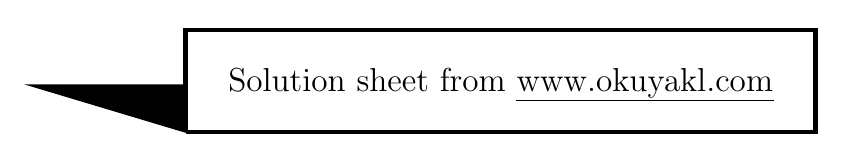
\begin{tikzpicture}(10,3)
		\draw[ultra thick](2,0) --(10,0) -- (10,1.3) --(2,1.3) -- (2,0);
		\draw[fill=black](2,0)-- (0,.6) -- (2,.6) -- (2,0);
		\node at (6,.6) {\large Solution sheet from \href{http://www.okuyakl.com}{www.okuyakl.com}};
	\end{tikzpicture}
	\vspace{0.5 cm}
	
	\noindent{\bf Task 1.}\\
	\begin{itemize}
		\item {\bf Heat conduction} occurs at the point where two bodies of different temperatures touch each other.
		\item {\bf Thermal radiation :} The surface of a warm body emits infrared radiation.
		\item {\bf Convection:} Heated liquid or gas rises and transports heat upwards.
	\end{itemize}
	
	\noindent{\bf Task 2. a)}\\
	The temperature curve of this substance has breakpoints at $\SI{0}{\celsius}$ and $\SI{100}{\celsius}$, so it is water.
	
	\noindent{\bf Task 2. b)}\\
	All terms describe phase transitions; the table must be read line by line.
	
	\renewcommand{\arraystretch}{2}
	\begin{tabular}{|c|c|c|c|}
		\hline
		Phase & solid & liquid & gaseous \\
		\hline
		solid & - & melt & sublimate \\
		\hline
		liquid & solidify & - & boil \\
		\hline
		gaseous & resublimate & condense & - \\
		\hline
	\end{tabular}
	\vspace{0.5 cm}
	
	\noindent{\bf Task 2. c)}\\
	\begin{itemize}
		\item {\bf Point A:} Solid phase: Ice is heated to the melting point
		\item {\bf Point B:} Melting process: During melting, the temperature remains at $273~K$ until there is no more ice.
		\item {\bf Point C:} Liquid phase: Water heats continuously to the boiling point.
		\item {\bf point D:} The water is boiling
		\item {\bf Point E:} All the water has evaporated, the steam now continues to heat up.
	\end{itemize}
	\vspace{0.5 cm}
	
	\noindent{\bf Task 3. a)}\\
	To melt the ice we need the amount of heat:
	$$Q_s = s_{H_2O}\cdot m = \SI{334}{\kilo\joule\over \kilogram} \cdot \SI{0.16}{\kilogram} = \SI{53.4}{\ kilo\joule}$$
	To heat the now liquid water you need:
	$$Q_c = c_{H_2O}\cdot m \cdot \Delta \vartheta = \SI{4.18}{\kilo\joule\over \kilogram\kelvin}\cdot \SI{0.16}{\kilogram} \cdot \SI{100}{\kelvin}= \SI{66.9}{\kilo\joule}$$
	The evaporation of water requires the amount of heat:
	$$Q_r = r_{H_2O}\cdot m = \SI{2257}{\kilo\joule\over \kilogram}\cdot \SI{0.16}{\kilogram} = \SI{361}{\kilo\joule}$$
	The amount of heat required to evaporate the ice is:
	$$Q_{ges}=Q_s + Q_c + Q_r = \SI{481}{\kilo\joule}$$
	\vspace{0.5 cm}
	
	\noindent{\bf Task 3. b)}\\
	Here the power is equal to the amount of heat per time and we transform:
	$$ P = {Q \over t} \quad \Rightarrow \quad t = {Q \over P} = {\SI{481e3}{\joule}\over \SI{2800}{\watt}}=\SI {172}{\second} $$
	The heating time is therefore around three minutes.
	\vspace{0.5 cm}
	
	\noindent{\bf Task 4. a)}\\
	A bimetallic strip consists of two layers of different metals, which also expand differently when heated. As a result, the strip bends in the direction of the metal with the smaller thermal expansion when it heats up, and in the other direction when it cools down.
	\vspace{0.5 cm}
	
	\noindent{\bf Task 4. b)}\\
	This is a thermostat, a switch usually installed in heating devices that turns them on when the temperature falls below a certain temperature and turns them off when the temperature exceeds a certain temperature.
	\vspace{0.5 cm}
	
	\noindent{\bf Task 5.}\\
	The room temperature of $\SI{19}{\celsius}$ in Kelvin is:
	$$T_K = T_C + 273.15 = 19 + 273.15 = \SI{292.15}{\kelvin} $$
	The boiling point of oxygen is $\SI{90}{\kelvin}$, so the air has to
	$$\SI{292,15}{\kelvin}- \SI{90}{\kelvin} \approx \SI{202}{\kelvin}$$
	be cooled to liquefy it.
	\vspace{0.5 cm}
	
	\noindent{\bf Task 6. a)}\\
	The amount of heat absorbed by the amount of water $m_2$ after condensation is:
	$$Q_2=c_{H_2O}\cdot m_2 \cdot (82-20)\SI{}{\kelvin} = \SI{4,2}{\kilo\joule\over \kilogram\kelvin}\cdot \SI {1.8}{\kilogram} \cdot \SI{62}{\kelvin} = 468~kJ$$
	\vspace{0.5 cm}
	
	\noindent{\bf Task 6. b)}\\
	The amount of heat given off by the $\SI{100}{\celsius}$ hot, condensed water of the amount $m_1$ is:
	$$Q_1=c_{H_2O}\cdot m_1 \cdot (100-82)\SI{}{\kelvin} = \SI{4,2}{\kilo\joule\over \kilogram\kelvin}\cdot \SI {0.2}{\kilogram} \cdot \SI{18}{\kelvin} = \SI{15}{\kilo\joule}$$
	The difference between these two values is the amount of heat released by the condensation of water vapor:
	$$Q_k= Q_2-Q_1=\SI{468}{\kilo\joule}-\SI{15}{\kilo\joule}=\SI{453}{\kilo\joule}$$
	After rearranging the formula we get for $r$:
	$$Q_k = r\cdot m \quad \Rightarrow\quad r= {Q_k \over m} =\SI{2265}{\kilo\joule\over \kilogram} \approx \SI{2,3e3}{\kilo\joule\over \kilogram} $$
	This value matches the literature value given above quite closely.
	\vspace{0.5 cm}
	
	\noindent{\bf Task 7.}\\
	The water-ice mixture now has the temperature $\SI{0}{\celsius}$. The following applies again: heat absorbed = heat released. The amount of water $m_w$ has given off the amount of heat:
	$$Q_w = c_{H_2O}\cdot m_w \cdot \Delta \vartheta =\SI{4,2}{\kilo\joule\over \kilogram\kelvin} \cdot \SI{3,2}{\kilogram} \cdot \SI{30}{\kelvin} = \SI{403}{\kilo\joule}$$
	The mass fraction of melted ice is:
	$$m_{ge}=0.70 \cdot \SI{1.5}{\kilogram}= \SI{1.05}{\kilogram}$$
	To melt this ice cream mass you needed:
	$$Q_s=s_w \cdot m_w = \SI{334}{\kilo\joule\over \kilogram} \cdot \SI{1.05}{\kilogram}=\SI{351}{\kilo\joule}$$
	The difference between the two amounts of heat results in the amount of heat absorbed by the solid ice:
	$$Q_e = Q_w-Q_s=\SI{52}{\kilo\joule}$$
	The ice was heated to the following temperature:
	$$
	\renewcommand{\arraystretch}{2}
	\begin{array}{rcll}
		Q_e &=& c_{eis}\cdot m_{eis}\cdot \Delta \vartheta &|\: c_{eis} \quad |: m_{eis}\\
		\Delta \vartheta &=& {Q_e \over c_{eis}\cdot m_{eis}}\\
		\Delta \vartheta &=& {\SI{52}{\kilo\joule}\over \SI{2,1}{\kilo\joule\cdot \kilogram^{-1}\cdot \kelvin^{-1 }}\cdot \SI{1.5}{\kilogram}}\\
		\Delta \vartheta &=& 17~K
	\end{array}
	$$
	The ice had a temperature of $\SI{-17}{\celsius}$ before it was added to the water.
	\vspace{0.5 cm}
	
	\noindent{\bf Task 8. a)}\\
	The metal of the spoon consists of an atomic lattice in which neighboring atoms touch each other. If you heat an area of this lattice, the atoms begin to oscillate more strongly around their rest position. Through collisions with neighboring atoms, these vibrations ultimately also affect more distant areas of the lattice.
	\vspace{0.5 cm}
	
	\noindent{\bf Exercise 8. b)}\\
	For example, convection occurs in a room with a radiator. An air parcel first heats up through contact with the warm surface of the radiator. The heated air rises due to its lower density and colder air reaches the radiator, which in turn is heated and rises. This creates a circulation through which the entire air in the room is gradually heated.
	\vspace{0.5 cm}
	
	\noindent{\bf Task 9.}\\
	The energy supplied is equal to the potential. This gives us:
	$$
	\renewcommand{\arraystretch}{2}
	\begin{array}{rcll}
		m_{ges}\cdot g \cdot h &=& c \cdot m_{br} \cdot \Delta \vartheta & |:c \quad |:m_{br} \\
		\Delta \vartheta &=& {m_{ges}\cdot g \cdot h \over c \cdot m_{br}} \\
		\Delta \vartheta &=& {\SI{85}{\kilogram} \cdot \SI{9,81}{\meter\over{\second^2}}\cdot \SI{100}{\meter} \over \SI{480}{\joule\cdot\kilogram^{-1}\cdot\kelvin^{-1}} \cdot \SI{1,0}{\kilogram}} \\
		\Delta \vartheta &=& \SI{174}{\kelvin}\\
	\end{array}
	$$
	The drum brake heats up to 174~K.
	\vspace{0.5 cm}
	
	\noindent{\bf Task 10.}\\
	In a closed system the sum of the energies is constant:
	internal energy = amount of heat + work
	$$E_i = Q + W$$
	\vspace{0.5 cm}
	
	\begin{center}
		\includegraphics[width=7 cm]{../../viecher/eendcomic.pdf}
		
		Here you can go back to the \href{https://www.okuyakl.de/phys/p9thaL402/ae402.pdf}{task sheet}
	\end{center}
	
	\end{document}